\section{Question 6}
Consider the following recurrent network. Assume that this network receives two sequences of zeros and ones and returns the number 1 if the two sequences are equal, and the number 0 otherwise.
\begin{figure}[H]
	\centering
	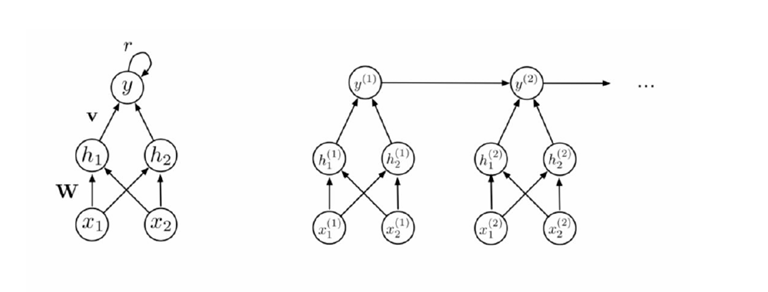
\includegraphics[width=0.8\textwidth]{Q6.png}
	\caption{Recurrent network}
\end{figure}
The matrix \(W\) is a \(2 \times 2\) matrix, and \(\mathbf{v}\), \(\mathbf{b}\) are 2-dimensional vectors, and \(c\), \(r\), and \(c_0\) are scalars. Determine these parameters so that the network operates as described. (Hint: \(y^{(t)}\), the output at time \(t\), indicates whether the two sequences have been equal up to that point. The first hidden layer indicates whether the two inputs at time \(t\) were both zero, and the second hidden layer indicates whether the two inputs at time \(t\) were both one.)

\[
h^{(t)} = \phi\left(W x^{(t)} + \mathbf{b}\right)
\]

\[
y^{(t)} =
\begin{cases} 
    \phi\left(\mathbf{v}^\top h^{(t)} + r y^{(t-1)} + c\right) & \text{for } t > 1 \\
    \phi\left(\mathbf{v}^\top h^{(t)} + c_0\right) & \text{for } t = 1
\end{cases}
\]

\[
\phi(z) = 
\begin{cases} 
    1 & \text{if } z > 0 \\
    0 & \text{if } z \leq 0
\end{cases}
\]
\begin{qsolve}
	\begin{qsolve}[]
		The hidden states \( h_1^{(t)} \) and \( h_2^{(t)} \) represent whether the two inputs \( x_1^{(t)} \) and \( x_2^{(t)} \) satisfy specific conditions at time \( t \):
		\begin{center}
		\( h_1^{(t)} \) indicates if both \( x_1^{(t)} = 0 \) and \( x_2^{(t)} = 0 \).

		\( h_2^{(t)} \) indicates if both \( x_1^{(t)} = 1 \) and \( x_2^{(t)} = 1 \).	
		\end{center}
		
To achieve this, we set the matrix \( W \) and bias \( \mathbf{b} \) as:
\splitqsolve[\splitqsolve]
\[
W = 
\begin{bmatrix}
-1 & -1 \\
1 & 1
\end{bmatrix}, \quad
\mathbf{b} = 
\begin{bmatrix}
1 \\
-1
\end{bmatrix}.
\]
This ensures that:
\[
h_1^{(t)} = \phi(-x_1^{(t)} - x_2^{(t)} + 1),
\]
which outputs \( 1 \) when \( x_1^{(t)} = 0 \) and \( x_2^{(t)} = 0 \), and \[ h_2^{(t)} = \phi(x_1^{(t)} + x_2^{(t)} - 1) \], which outputs \( 1 \) when \( x_1^{(t)} = 1 \) and \( x_2^{(t)} = 1 \).

The output \( y^{(t)} \) should indicate whether the inputs have been equal up to time \( t \). For \( t = 1 \), the output depends only on the initial hidden state:
\[
y^{(1)} = \phi(\mathbf{v}^\top h^{(1)} + c_0),
\]
where \( \mathbf{v} = \begin{bmatrix} 1 \\ 1 \end{bmatrix} \) and \( c_0 = -0.5 \). This ensures \( y^{(1)} = 1 \) if \( h_1^{(1)} + h_2^{(1)} = 1 \) (i.e., \( x_1^{(1)} = x_2^{(1)} \)), and \( y^{(1)} = 0 \) otherwise.

For \( t > 1 \), \( y^{(t)} \) depends on both the current hidden state \( h^{(t)} \) and the previous output \( y^{(t-1)} \). The equation is:
\[
y^{(t)} = \phi(\mathbf{v}^\top h^{(t)} + r y^{(t-1)} + c),
\]
where \( r = 2 \) and \( c = -2.5 \). This ensures that \( y^{(t)} = 1 \) if the inputs match at time \( t \) and \( y^{(t-1)} = 1 \), maintaining consistency across all time steps.

as an example Consider the input sequences:
\[
x_1 = [1, 1, 0, 0, 1], \quad x_2 = [1, 1, 0, 0, 0].
\]

At each time step:

- \( h_1^{(t)} = 1 \) if \( x_1^{(t)} = 0 \) and \( x_2^{(t)} = 0 \),

- \( h_2^{(t)} = 1 \) if \( x_1^{(t)} = 1 \) and \( x_2^{(t)} = 1 \),

- \( y^{(t)} = 1 \) only if \( x_1 \) and \( x_2 \) have been equal up to time \( t \).

The outputs are computed as follows:
\[
h_1 = [0, 0, 1, 1, 0], \quad h_2 = [1, 1, 0, 0, 0],
\]
\[
y = [1, 1, 1, 1, 0].
\]

The final output sequence is:
\[
y = [1, 1, 1, 1, 0].
\]
	\end{qsolve}
\end{qsolve}